% 4.methodology.tex — TEMPO Methodology

\begin{figure*}[!t]
    \centering
    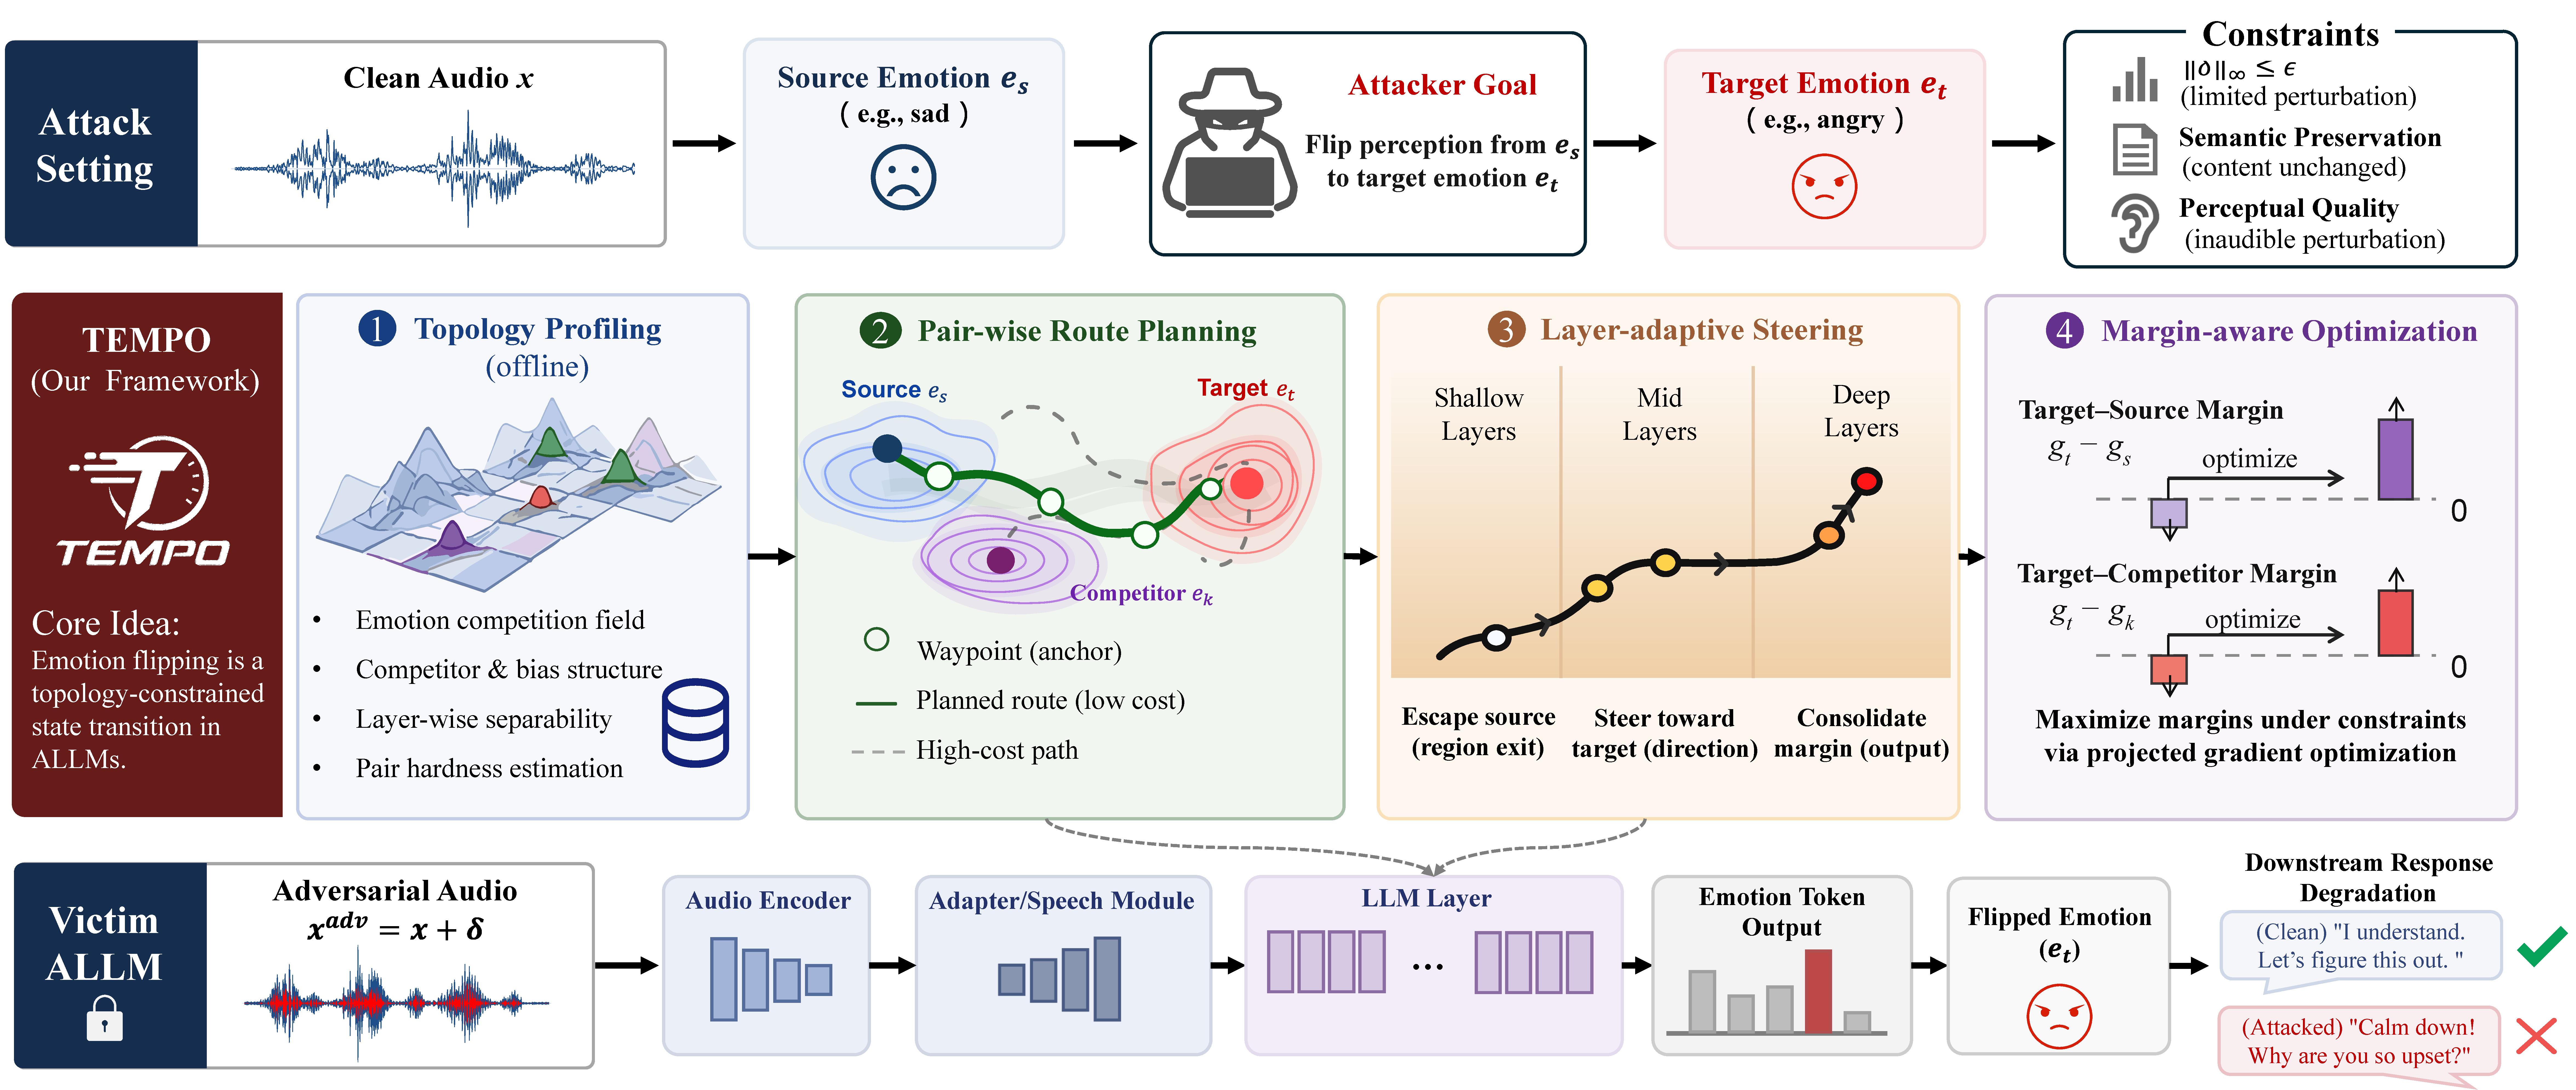
\includegraphics[width=\textwidth]{figure/figuretempo_overview.pdf}
    \caption{\textbf{Overview of \textsc{TEMPO}.} \textsc{TEMPO} converts clean-side observations into a topology prior, plans a pair-specific transition route, and optimizes adversarial audio through layer-adaptive control and margin-aware scheduling. The attack is not a one-step target-token maximization problem; it is a controlled transition that escapes the source region, follows a feasible route, and consolidates target dominance under semantic and perceptual constraints.}
    \label{fig:tempo-overview}
\end{figure*}

\section{TEMPO: Topology-Guided Emotion Manipulation by Pairwise Optimization}
\label{sec:method-tempo}

We present \textsc{TEMPO}, a topology-guided framework for controllable emotion flipping in Audio LLMs. The threat model in Section~\ref{sec:threat_model} identifies three structural challenges: the emotion decision interface is implicit and competition-based, source--target transitions are pair-dependent, and the effective control bottleneck lies inside the model rather than only at the output. TEMPO is designed around these challenges. Instead of treating the attack as direct target-token maximization, it treats emotion manipulation as a structured state transition in the model's internal affective space.

At a high level, a successful transition must satisfy three conditions. First, the representation must leave the source emotion region. Second, it must move along a feasible source-to-target route rather than collapse into a model-specific attractor or competitor. Third, the target emotion must dominate both the source and the strongest competitor at the output interface. Figure~\ref{fig:tempo-overview} summarizes this workflow. TEMPO first profiles the model-specific emotion topology, then estimates pair-wise transition hardness, selects a direct or waypoint-assisted route, and finally realizes this route through layer-adaptive and margin-aware optimization.

\subsection{Topology Bank: Modeling the Emotion Competition Field}
\label{subsec:tempo-topology}

To address the implicit competition interface in C1, TEMPO first constructs a model-specific topology bank. The purpose of this component is to turn a hidden, open-vocabulary emotion decision process into an explicit attack prior. Without such a prior, the attacker only observes that a target token should be increased, but does not know which non-target emotion competes with it, which bias center the model naturally falls back to, or which internal layer exposes the most controllable emotion boundary.

Figure~\ref{fig:tempo-topology-field} illustrates the abstraction. The source emotion $e_s$ is not isolated: it lies in a competition field that also contains the attacker-chosen target $e_t$, the dominant competitor $k_m(s)$, and the model-specific bias center $b_m$. The role of the topology bank is to summarize this field in a compact form that later modules can use for route planning and representation control.

\begin{figure}[!t]
    \centering
    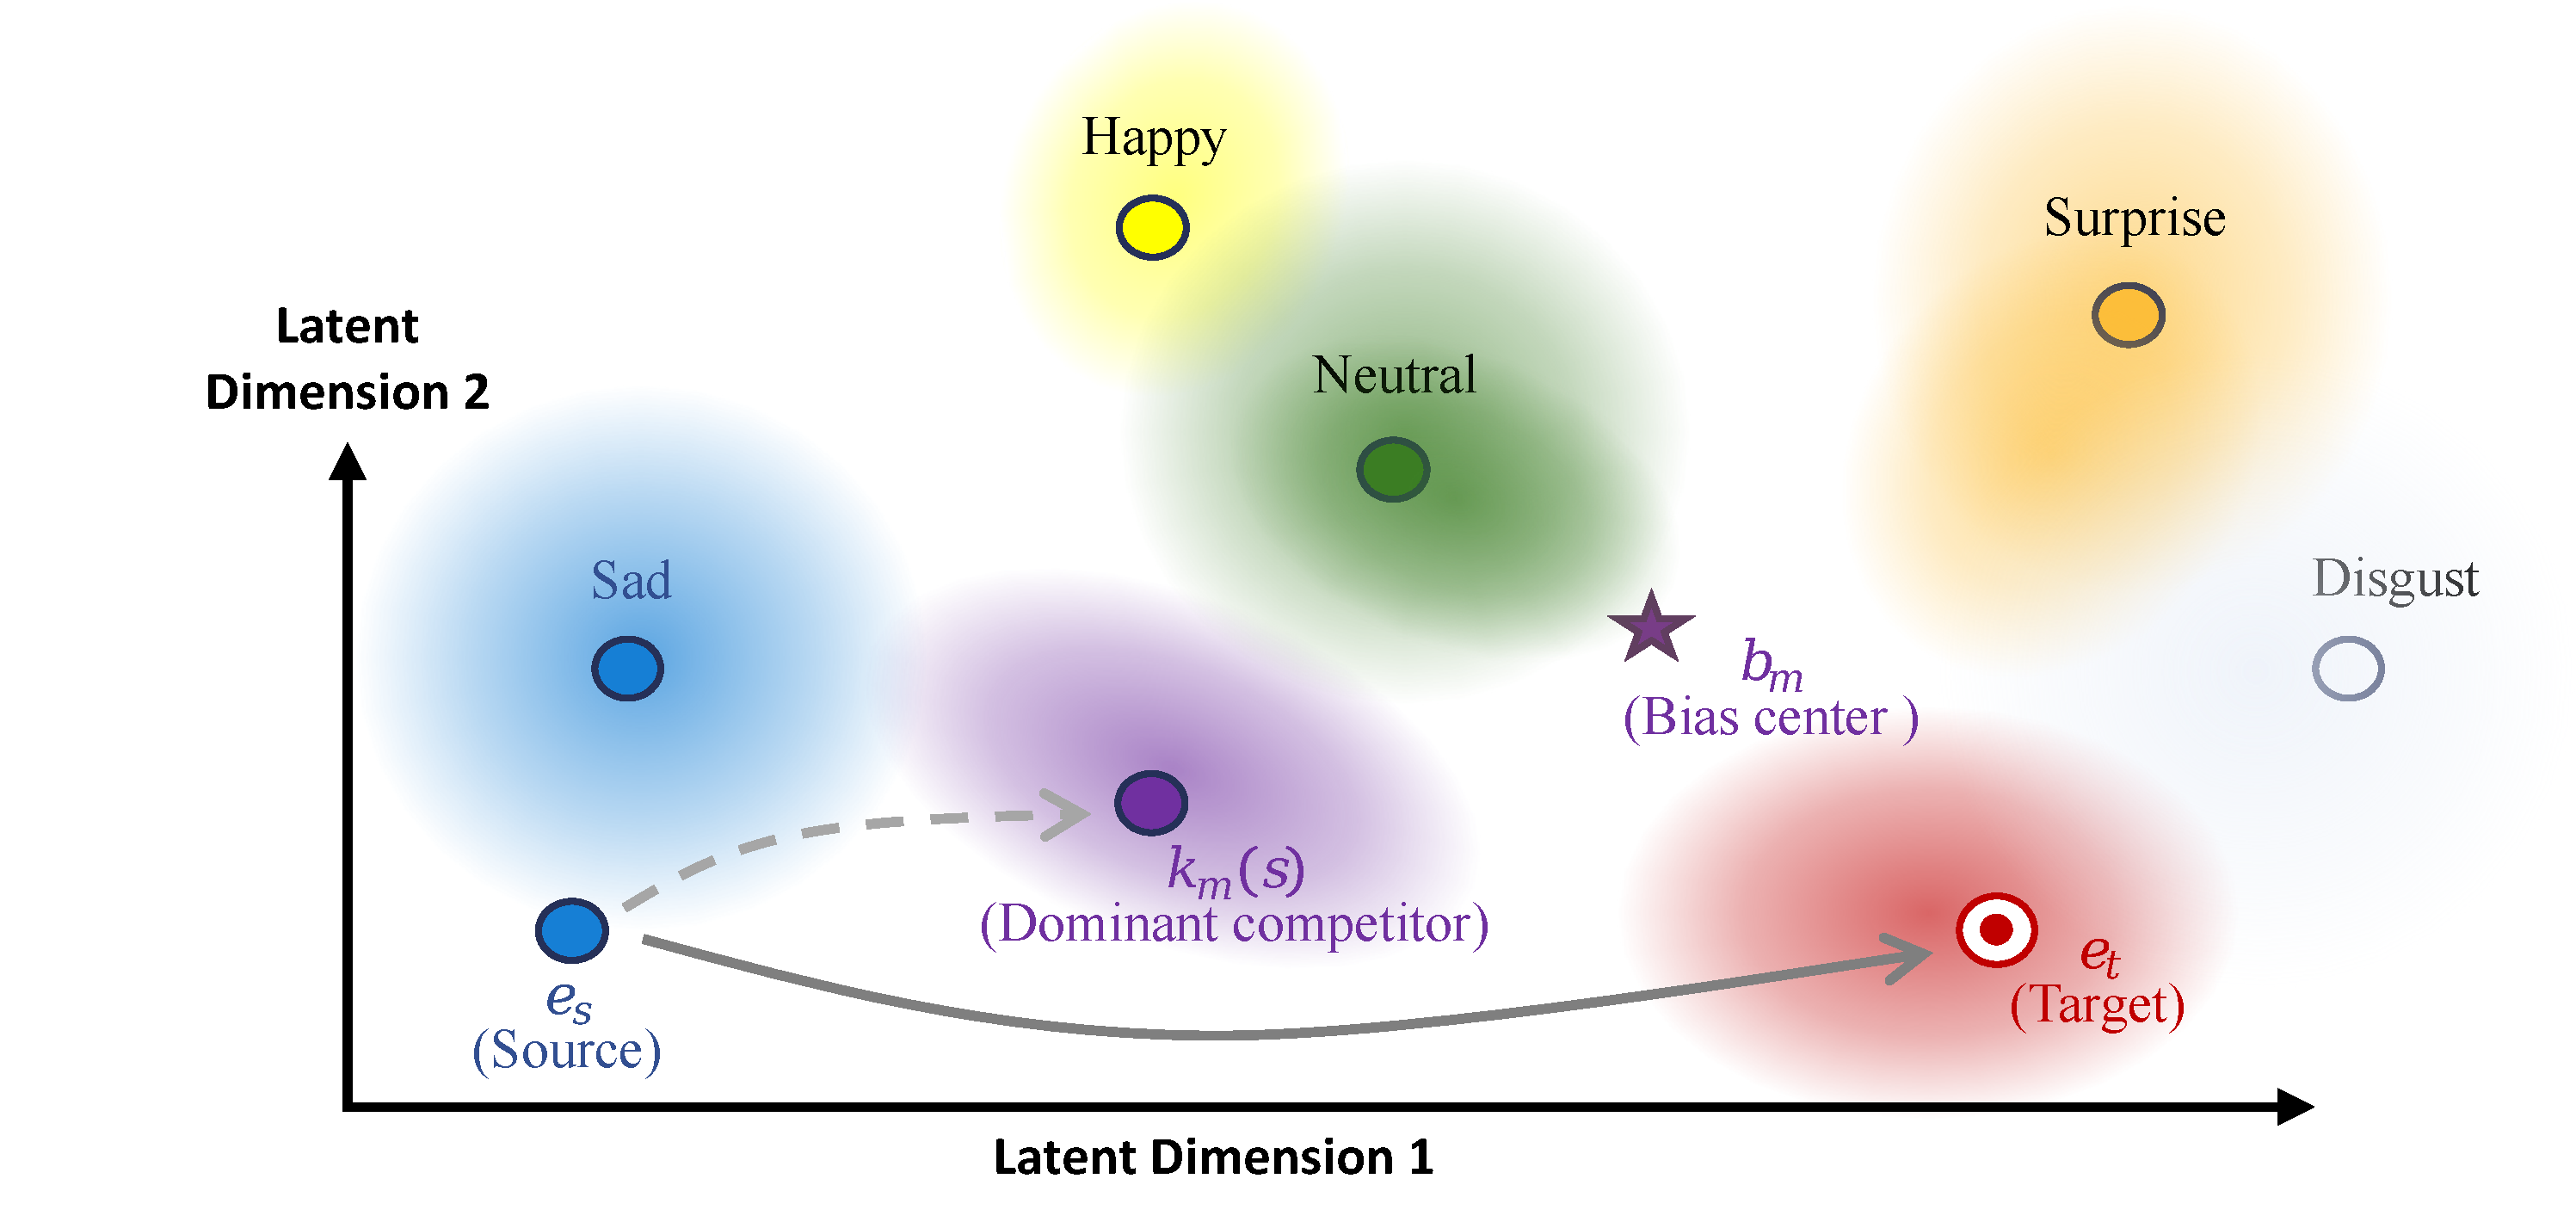
\includegraphics[width=\linewidth]{figure/fig7a_topology_field.pdf}
    \caption{\textbf{Abstract emotion competition field.} The source emotion $e_s$ competes with a dominant competitor $k_m(s)$ and the attacker-chosen target $e_t$. The attack objective is therefore not merely to increase the target score, but to overcome the model's natural competition bias.}
    \label{fig:tempo-topology-field}
\end{figure}

For each model $m$, we define the topology bank as
\begin{equation}
\mathcal{B}_m =
\left\{
 b_m,\;
 k_m(e),\;
 l^{m}_{\mathrm{mid}},\;
 l^{m}_{\mathrm{deep}},\;
 \mu_{m,l,e},\;
 H_m(s,t)
\right\}.
\label{eq:topology-bank}
\end{equation}
Here $b_m$ is the dominant bias center, $k_m(e)$ is the strongest competitor of emotion $e$, $l^{m}_{\mathrm{mid}}$ and $l^{m}_{\mathrm{deep}}$ are the preferred boundary and steering layers, $\mu_{m,l,e}$ is the prototype of emotion $e$ at layer $l$, and $H_m(s,t)$ estimates the hardness of moving from source $s$ to target $t$.

The bank is obtained from clean probing. We query the model with emotion-elicitation prompts, collect first-step emotion scores over the candidate emotion set, and estimate source-dependent competitors from the highest non-source alternatives. We then compute hidden-state prototypes by pooling emotion-conditioned representations at each layer and selecting the layers that show strong mid-layer separability. Finally, we estimate pair-wise hardness from the competition statistics and prototype geometry. In this way, the topology bank preserves both shared structure and model-specific differences: the existence of emotion competition is shared across models, while the bias center, competitor relation, and hard transitions differ by architecture.

This component resolves C1 by replacing an implicit decoding interface with an explicit competition model. The rest of TEMPO does not optimize toward the target in isolation; it uses $\mathcal{B}_m$ to decide which competitor must be suppressed, which internal layers should be controlled, and which source--target transitions require special handling.

\subsection{Pair-wise Hardness and Route Planning}
\label{subsec:tempo-route}

To address the pair-dependent transition difficulty in C2, TEMPO plans an attack route before optimizing the waveform. The central issue is that emotion flips are not symmetric and not equally feasible. A direct transition may be easy when the target aligns with the model's bias structure, but hard when the path crosses a high-cost boundary or passes near a dominant competitor. A target-only objective ignores this geometry and can pull the representation into the model's default attractor instead of the intended target.

We therefore estimate a normalized pair-wise hardness matrix $H_m(s,t)$, as shown in Figure~\ref{fig:tempo-hardness}. The matrix acts as a cost landscape over the emotion topology: each entry quantifies how difficult it is to move from source $s$ to target $t$ under model $m$. The asymmetry of $H_m$ is important. A transition from $s$ to $t$ can be hard even if the reverse transition is easy, because the source margin, target basin, and dominant competitor are different in the two directions.

\begin{figure}[!t]
    \centering
    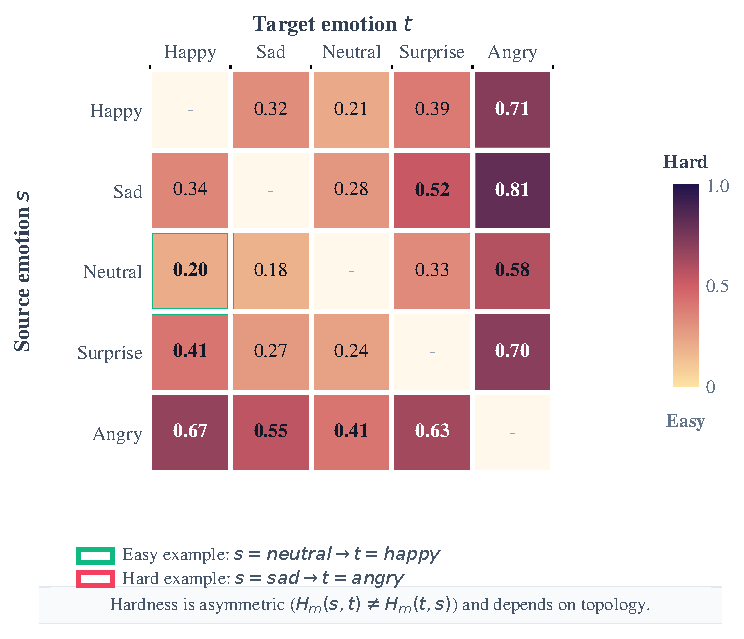
\includegraphics[width=\linewidth]{figure/fig7b_hardness_matrix.pdf}
    \caption{\textbf{Pair-wise attack hardness.} $H_m(s,t)$ quantifies how difficult it is to flip a source emotion $s$ into a target emotion $t$. The hardness is asymmetric and pair-dependent, motivating pair-specific route planning.}
    \label{fig:tempo-hardness}
\end{figure}

Given a sample $(x,s,t)$, TEMPO chooses either a direct route or a waypoint-assisted route:
\begin{equation}
\pi(s,t)=
\begin{cases}
(s,t), & \text{if } H_m(s,t)\le \tau_h \text{ or } t \in \{b_m, k_m(s)\},\\[1mm]
(s,u^\star,t), & \text{otherwise},
\end{cases}
\label{eq:tempo-route}
\end{equation}
where $\tau_h$ is a hardness threshold. The first case covers transitions that are already feasible or naturally aligned with the model's bias and competitor structure. The second case handles hard pairs by inserting an intermediate waypoint $u^\star$:
\begin{equation}
u^\star
=
\arg\min_{u\in \mathcal{E}\setminus\{s,t\}}
\Big(
D_m(s,u)+D_m(u,t)-\gamma\cdot \mathbb{I}[u=b_m]
\Big).
\label{eq:tempo-waypoint}
\end{equation}
Here $\mathcal{E}$ is the candidate emotion set, $D_m(\cdot,\cdot)$ is a topology distance derived from prototype separation and competition cost, and $\gamma$ controls whether the model's bias center is allowed to serve as a low-cost anchor. The waypoint is not introduced to change the final target; it is used only to decompose a difficult global transition into feasible local movements.

Figure~\ref{fig:tempo-route-example} visualizes this policy. Easy pairs follow a direct path, while hard pairs use an intermediate node to bypass a competitor barrier or high-cost region. This makes route planning a bridge between topology profiling and gradient optimization: the topology bank identifies the cost landscape, and the route policy converts it into a concrete sequence of control targets.

\begin{figure}[!t]
    \centering
    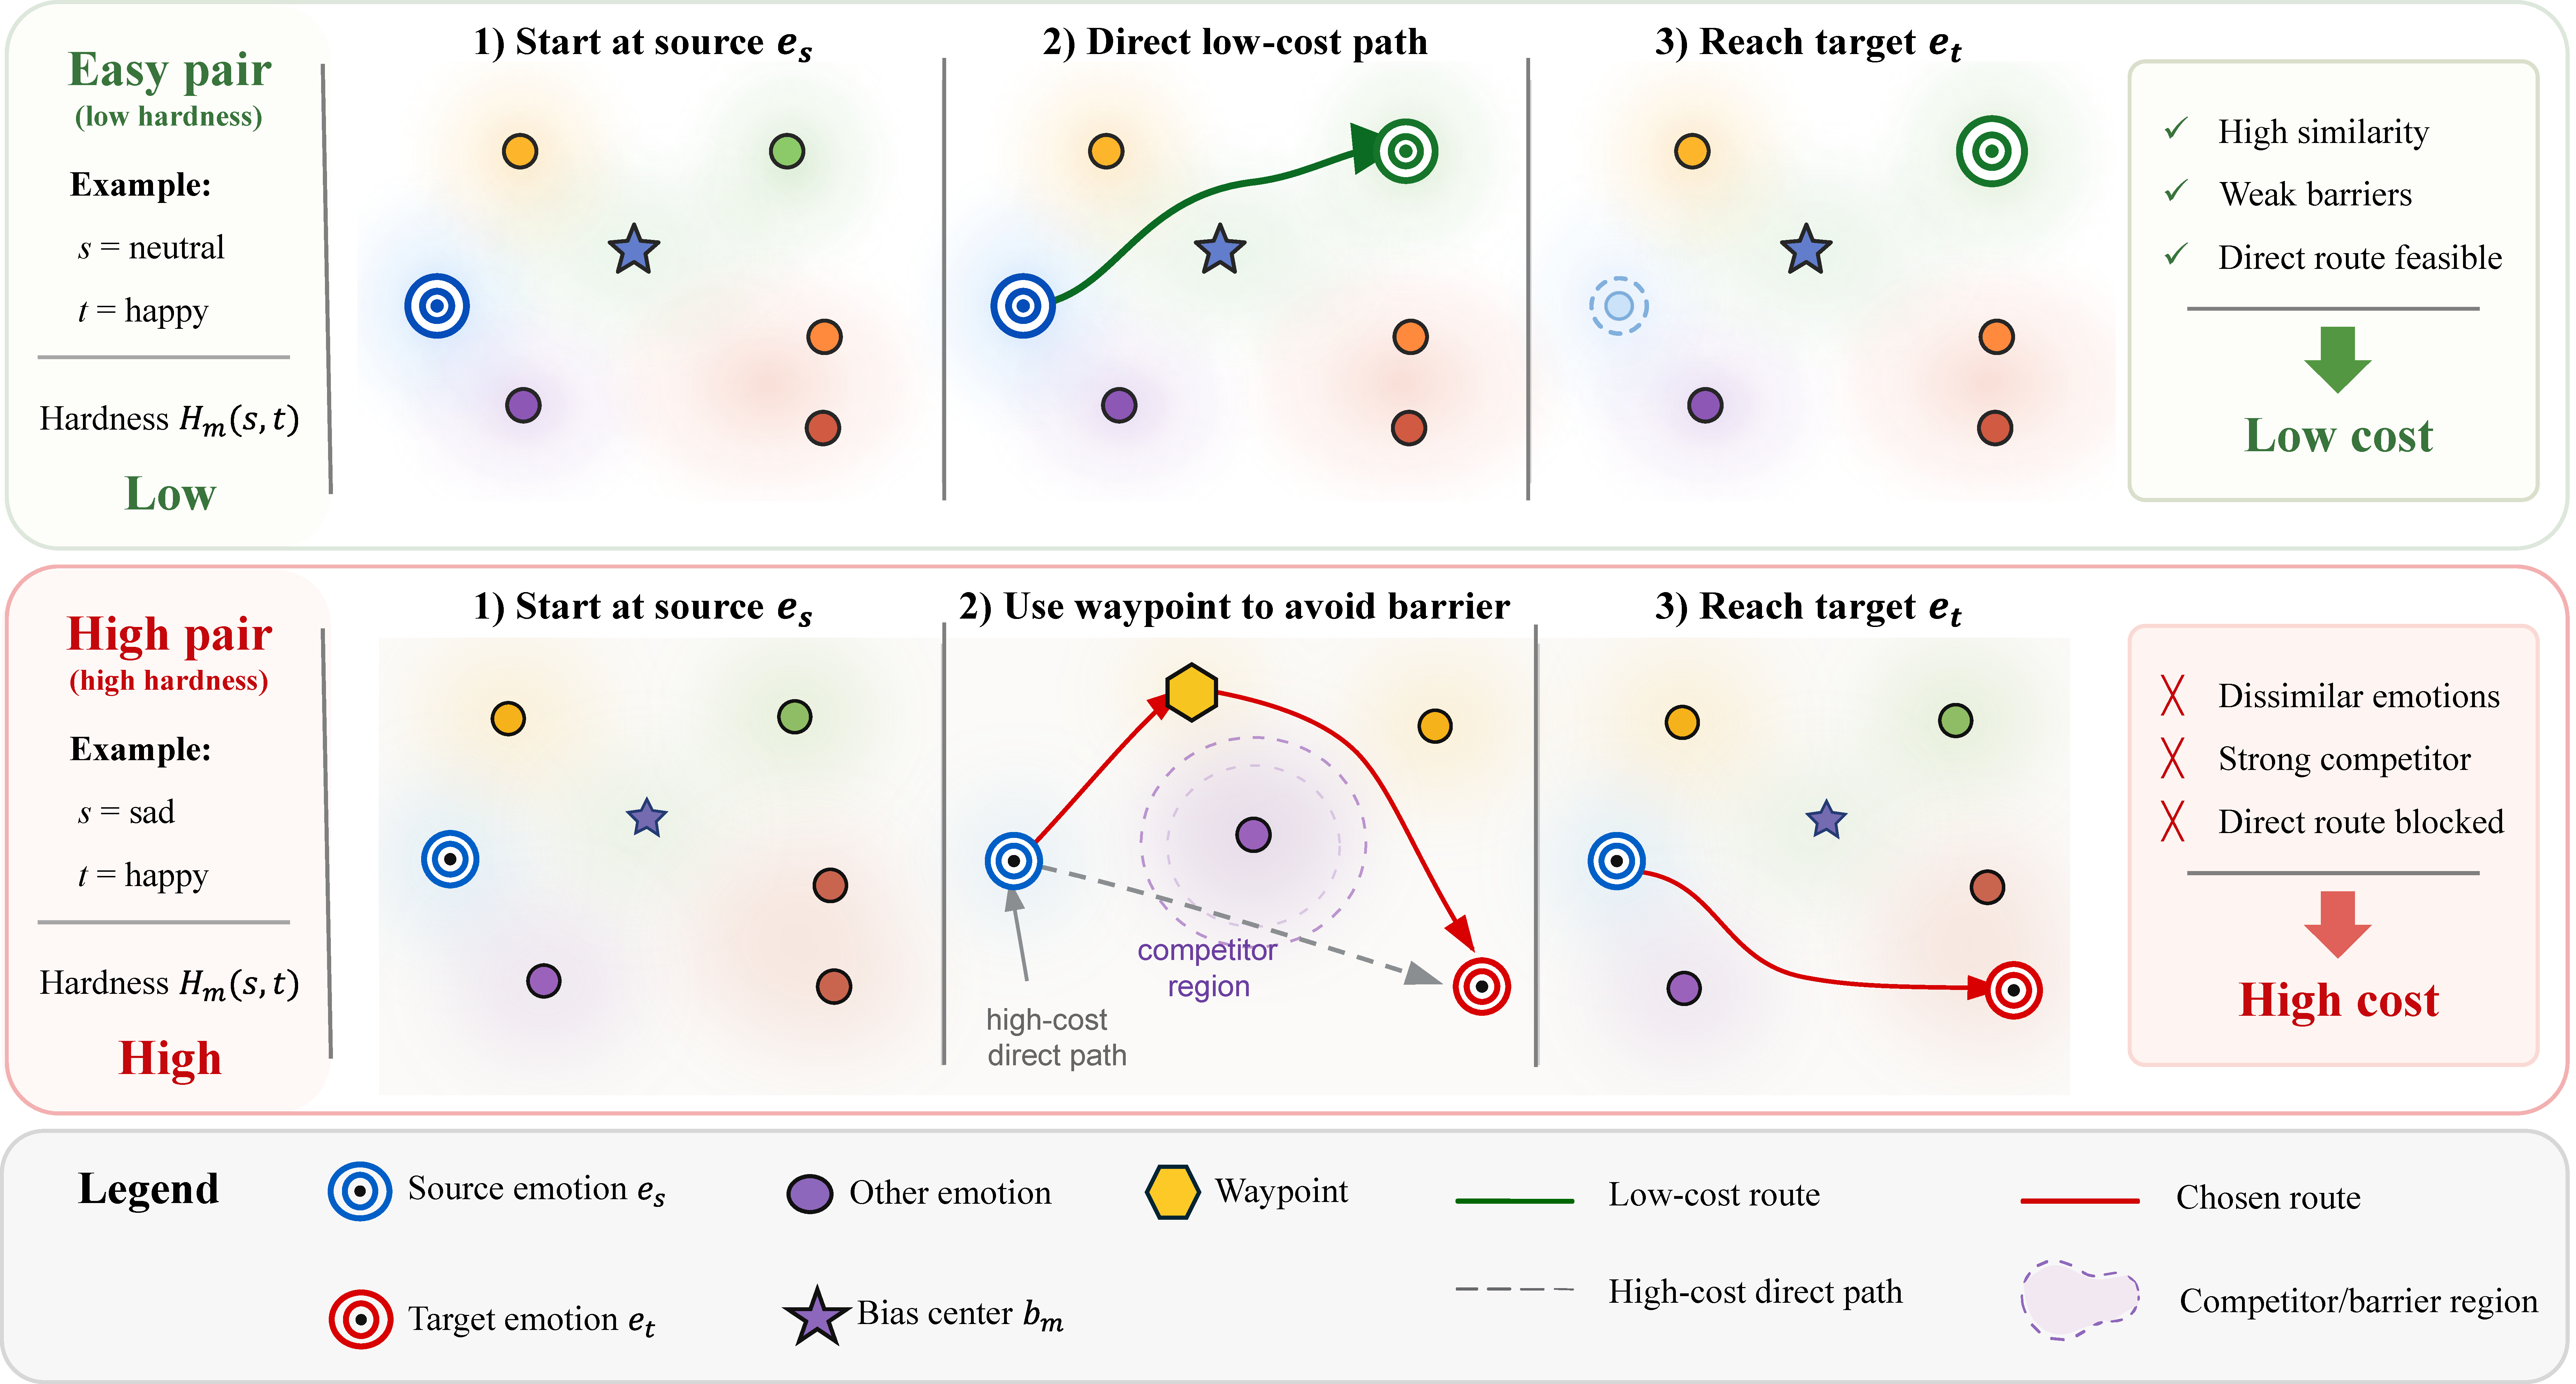
\includegraphics[width=\linewidth]{figure/fig7c_route_planning.pdf}
    \caption{\textbf{Topology-aware route planning.} Easy pairs follow a direct transition, while hard pairs use a waypoint-assisted route to avoid collapse into the dominant competitor or bias center.}
    \label{fig:tempo-route-example}
\end{figure}

This component resolves C2 by making the attack pair-specific. Rather than applying the same objective to all source--target pairs, TEMPO first asks whether the intended transition is topologically feasible. If not, it rewrites the attack as a sequence of local transitions that are easier to realize under a bounded perturbation budget.

\subsection{Layer-Adaptive Control Objectives}
\label{subsec:tempo-objective}

To address the internal control bottleneck in C3, TEMPO realizes the planned route through layer-adaptive control objectives. The route policy specifies where the representation should go, but not how to move it inside the model. Since Section~\ref{sec:obs-allm-universal} shows that emotion separability peaks at intermediate depth, controlling only the final output logits is insufficient. TEMPO therefore controls two levels simultaneously: intermediate representations are used to escape and steer, while first-step emotion scores are used to consolidate the final decision.

Let $h_l(x)$ denote the pooled hidden state at layer $l$, and let $g_e(x)$ denote the aggregated first-step score of emotion $e$. For a route whose current transition is $s\rightarrow u$ and final target is $t$, TEMPO uses three objectives corresponding to the three phases in Figure~\ref{fig:tempo-layer-control}: boundary exit, directional steering, and competition consolidation.

\begin{figure}[!t]
    \centering
    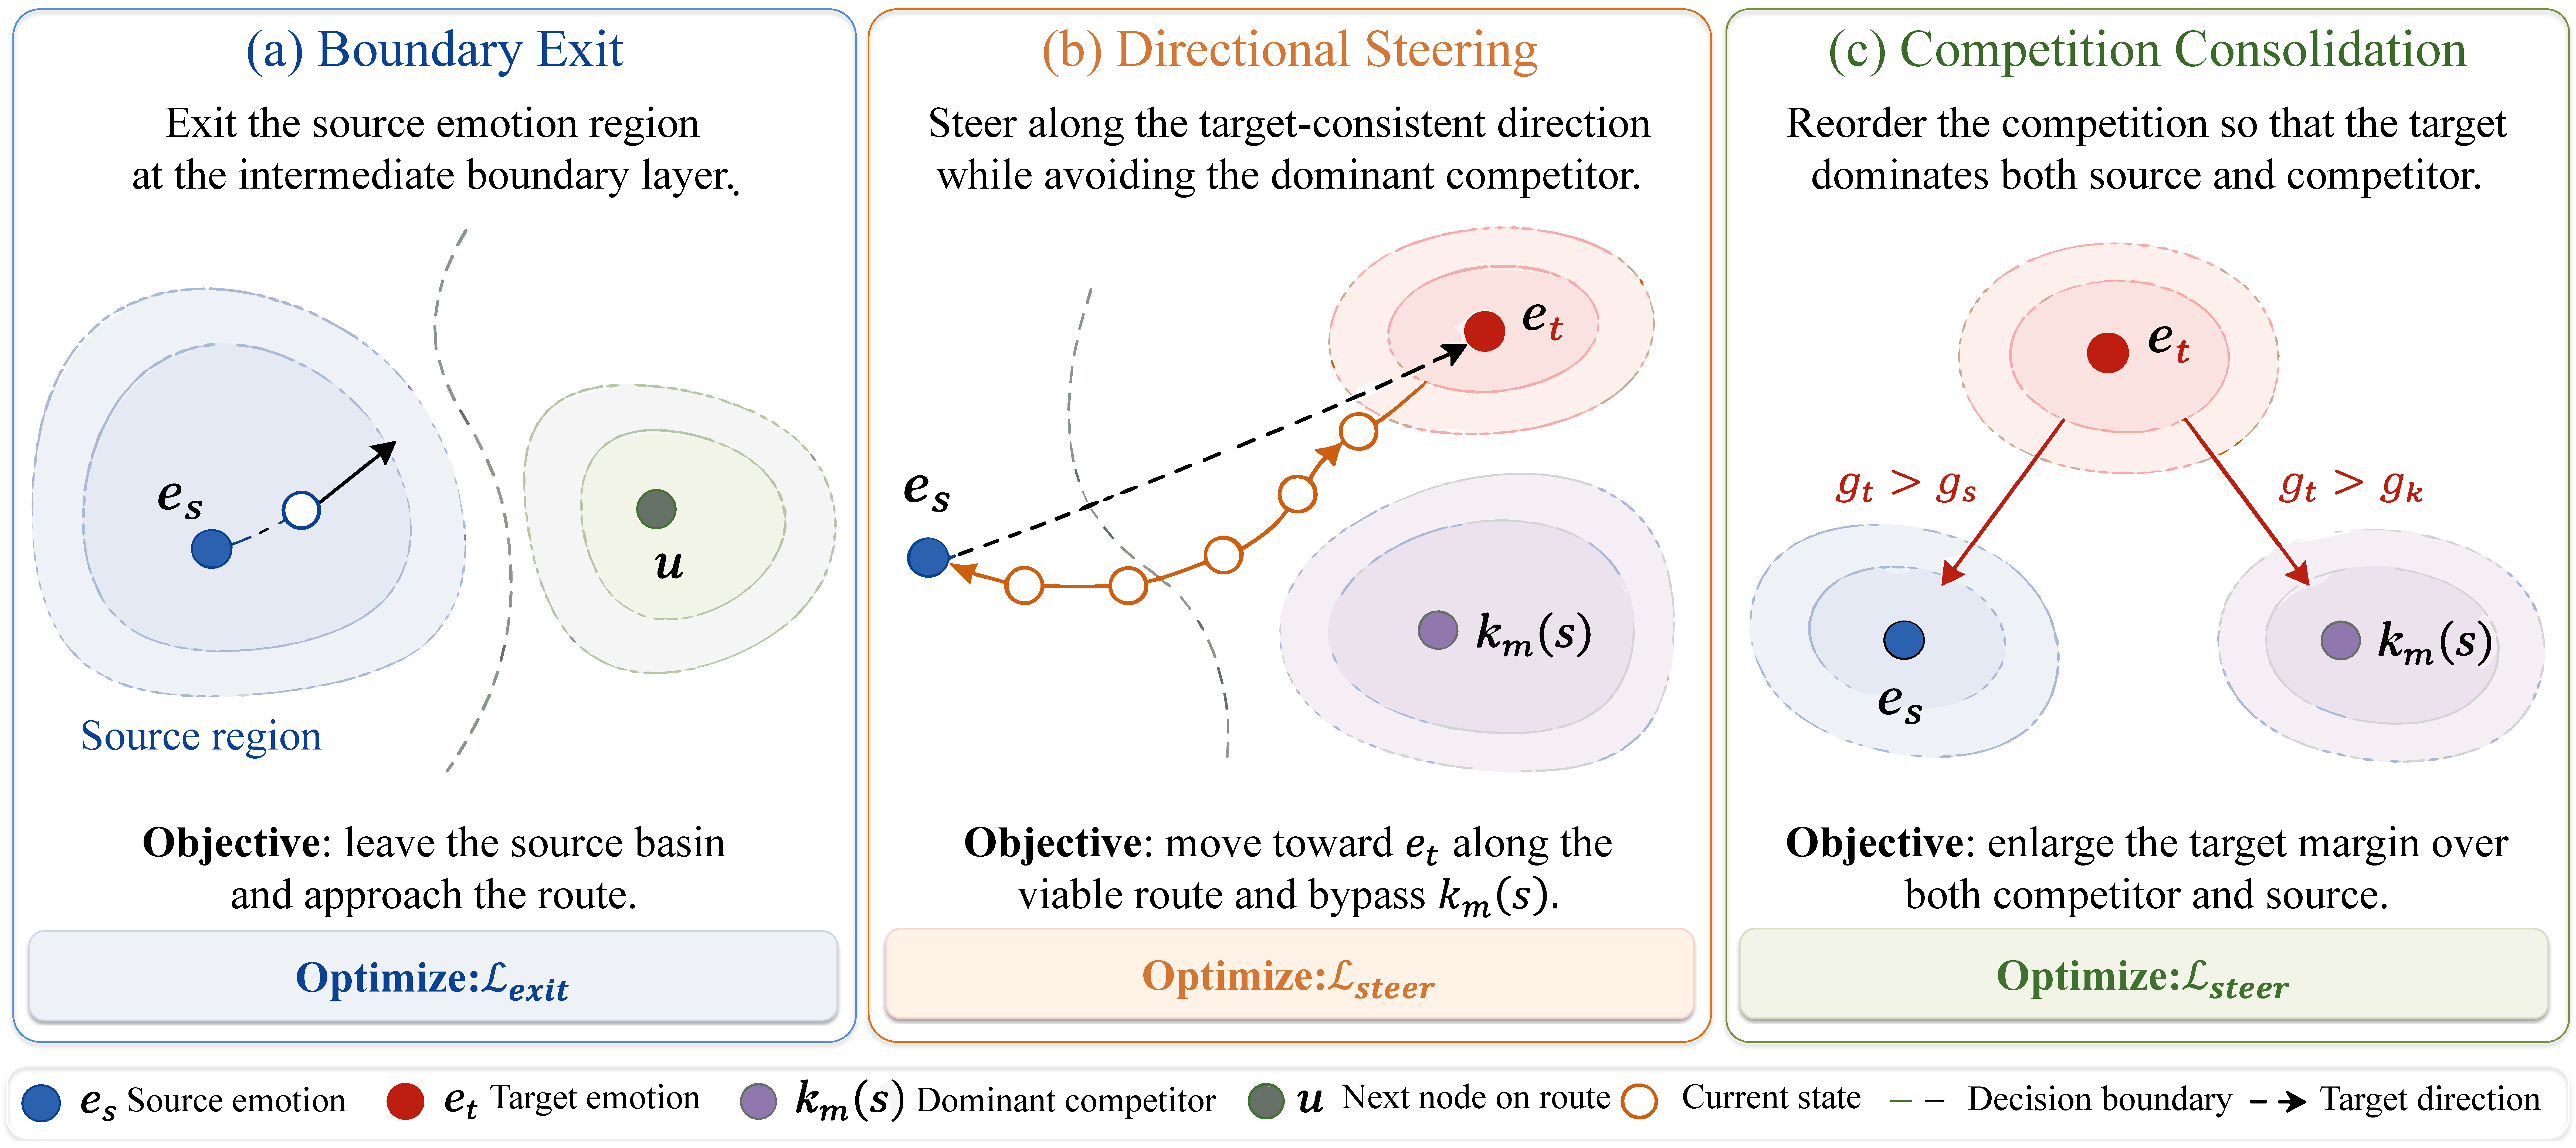
\includegraphics[width=\linewidth]{figure/fig8_layer_control.pdf}
    \caption{\textbf{Multi-phase control in \textsc{TEMPO}.} The attack first exits the source region, then steers the representation along a target-consistent direction, and finally consolidates the target by reordering the output competition margins.}
    \label{fig:tempo-layer-control}
\end{figure}

\paragraph{Boundary exit.}
The first step is to leave the source emotion basin. At the intermediate boundary layer $l^{m}_{\mathrm{mid}}$, TEMPO pushes the adversarial representation toward the next route node $u$ and away from the source prototype:
\begin{equation}
\mathcal{L}_{\mathrm{exit}}
=
\left\|h_{l^{m}_{\mathrm{mid}}}(x+\delta)-\mu_{m,l^{m}_{\mathrm{mid}},u}\right\|_2^2
-
\left\|h_{l^{m}_{\mathrm{mid}}}(x+\delta)-\mu_{m,l^{m}_{\mathrm{mid}},s}\right\|_2^2.
\label{eq:tempo-exit}
\end{equation}
Minimizing this term decreases the distance to the next node while increasing the relative distance from the source. This phase is necessary because a representation that remains inside the source basin can still decode as the source even if the target score is locally increased.

\paragraph{Directional steering.}
For hard pairs, escaping the source basin is not enough; the representation must move along a direction consistent with the planned route. TEMPO defines a normalized steering direction at the deeper control layer $l^{m}_{\mathrm{deep}}$:
\begin{equation}
d_{s\rightarrow u}
=
\frac{\mu_{m,l^{m}_{\mathrm{deep}},u}-\mu_{m,l^{m}_{\mathrm{deep}},s}}
{\left\|\mu_{m,l^{m}_{\mathrm{deep}},u}-\mu_{m,l^{m}_{\mathrm{deep}},s}\right\|_2},
\label{eq:tempo-direction}
\end{equation}
and optimizes
\begin{equation}
\mathcal{L}_{\mathrm{steer}}
=
-\left\langle
h_{l^{m}_{\mathrm{deep}}}(x+\delta)-h_{l^{m}_{\mathrm{deep}}}(x),\;
 d_{s\rightarrow u}
\right\rangle.
\label{eq:tempo-steer}
\end{equation}
This term rewards movement in the route-aligned direction and discourages uncontrolled representation drift. It is especially important for hard transitions where a perturbation can otherwise leave the source region but fall into a nearby competitor region.

\paragraph{Competition consolidation.}
The final step is to make the target emotion win the output-level competition. Let $k=k_m(s)$ be the dominant competitor of the source emotion. TEMPO uses a margin objective that requires the target to dominate both the source and this competitor:
\begin{equation}
\begin{aligned}
\mathcal{L}_{\mathrm{comp}}
={}&
\left[m_1 - \big(g_t(x+\delta)-g_s(x+\delta)\big)\right]_+
\\
&+
\left[m_2 - \big(g_t(x+\delta)-g_k(x+\delta)\big)\right]_+,
\end{aligned}
\label{eq:tempo-comp}
\end{equation}
where $m_1,m_2>0$ are safety margins and $[z]_+=\max(z,0)$. The first margin ensures that the target surpasses the source; the second ensures that it also surpasses the strongest non-source competitor. This is the step that distinguishes stable targeted flipping from transient target-score increase.

\paragraph{Overall objective.}
The complete loss is
\begin{equation}
\mathcal{L}
=
\lambda_c \mathcal{L}_{\mathrm{comp}}
+
\lambda_e \mathcal{L}_{\mathrm{exit}}
+
\lambda_d \mathcal{L}_{\mathrm{steer}}
+
\mathcal{L}_{\mathrm{pres}},
\label{eq:tempo-overall}
\end{equation}
where $\lambda_c$, $\lambda_e$, and $\lambda_d$ balance competition, exit, and steering, and $\mathcal{L}_{\mathrm{pres}}$ constrains semantic and perceptual distortion. We instantiate the preservation term as
\begin{equation}
\mathcal{L}_{\mathrm{pres}}
=
\lambda_{\mathrm{stft}}\mathcal{L}_{\mathrm{stft}}
+
\lambda_{\mathrm{asr}}\left[\tau-S_{\mathrm{asr}}(x,\delta)\right]_+,
\label{eq:tempo-preservation}
\end{equation}
where $\mathcal{L}_{\mathrm{stft}}$ is a multi-resolution STFT magnitude loss, and $S_{\mathrm{asr}}(x,\delta)$ denotes the sentence-level similarity between $\mathrm{ASR}_{f}(x+\delta,p_{\mathrm{asr}})$ and $\mathrm{ASR}_{f}(x,p_{\mathrm{asr}})$. The second term penalizes semantic drift below threshold $\tau$.

Together, these objectives resolve C3 by aligning the optimization with where emotion is actually controlled. TEMPO does not wait until decoding to force a label change. It first changes the internal state, then uses output margins to make the new state dominate the verbalized emotion decision.

\subsection{Margin-Aware Multi-Phase Optimization}
\label{subsec:tempo-optimization}

The preceding objectives define what the attack should optimize; the remaining question is how to allocate optimization effort. The same route does not require the same budget for every sample. If the clean source margin is large, the source decision is harder to escape. If the pair-wise hardness is high, the route is harder to realize. A fixed schedule can therefore be wasteful for easy samples and insufficient for hard samples. TEMPO uses margin-aware multi-phase optimization to adapt the perturbation budget and objective weights to the transition difficulty.

We first define the clean source-target margin:
\begin{equation}
M(x;s,t)=g_s(x)-g_t(x).
\label{eq:tempo-source-margin}
\end{equation}
The per-sample budget is then modulated by both normalized pair hardness and normalized clean margin:
\begin{equation}
\epsilon(x,s,t)
=
\epsilon_0
\left(
1+\alpha\,\widehat{H}_m(s,t)+\beta\,\widehat{M}(x;s,t)
\right),
\label{eq:tempo-budget}
\end{equation}
subject to the global maximum allowed by the threat model. Here $\epsilon_0$ is the base budget, $\widehat{H}_m$ and $\widehat{M}$ are normalized hardness and margin terms, and $\alpha,\beta$ control their influence. This schedule assigns more effort to structurally hard transitions and samples with strong clean-source dominance.

Optimization then proceeds in three phases:
\begin{align}
\mathcal{L}^{(1)} &= \lambda_e \mathcal{L}_{\mathrm{exit}} + \mathcal{L}_{\mathrm{pres}},
\label{eq:tempo-phase1}\\
\mathcal{L}^{(2)} &= \lambda_e \mathcal{L}_{\mathrm{exit}} + \lambda_d \mathcal{L}_{\mathrm{steer}} + \mathcal{L}_{\mathrm{pres}},
\label{eq:tempo-phase2}\\
\mathcal{L}^{(3)} &= \lambda_c \mathcal{L}_{\mathrm{comp}} + \lambda_d \mathcal{L}_{\mathrm{steer}} + \mathcal{L}_{\mathrm{pres}}.
\label{eq:tempo-phase3}
\end{align}
Phase I emphasizes boundary exit, because early optimization must first move the representation out of the source basin. Phase II adds directional steering, because the representation should follow the planned route rather than drift toward a competitor. Phase III emphasizes competition consolidation, because the final decision requires target dominance over both source and competitor.

At each step, TEMPO updates $\delta$ by projected gradient optimization and clips the result to the allowed $L_\infty$ ball. For robustness, the emotion score $g_e$ can be aggregated over multiple emotion-elicitation prompts, and expectation-over-transformation augmentation can be applied when evaluating physical or replay-based settings. These implementation choices do not change the objective; they make the optimized perturbation less tied to one prompt or channel realization.

Figure~\ref{fig:tempo-margin-dynamics} illustrates the intended dynamics. The target-source margin $g_t-g_s$ crossing zero indicates that the attack has escaped the source decision. The target-competitor margin $g_t-g_k$ crossing zero indicates stable target dominance. The success rate rises sharply only after both margins are reordered, confirming that reliable emotion flipping requires competition-aware consolidation rather than target-only score maximization.

\begin{figure}[!t]
    \centering
    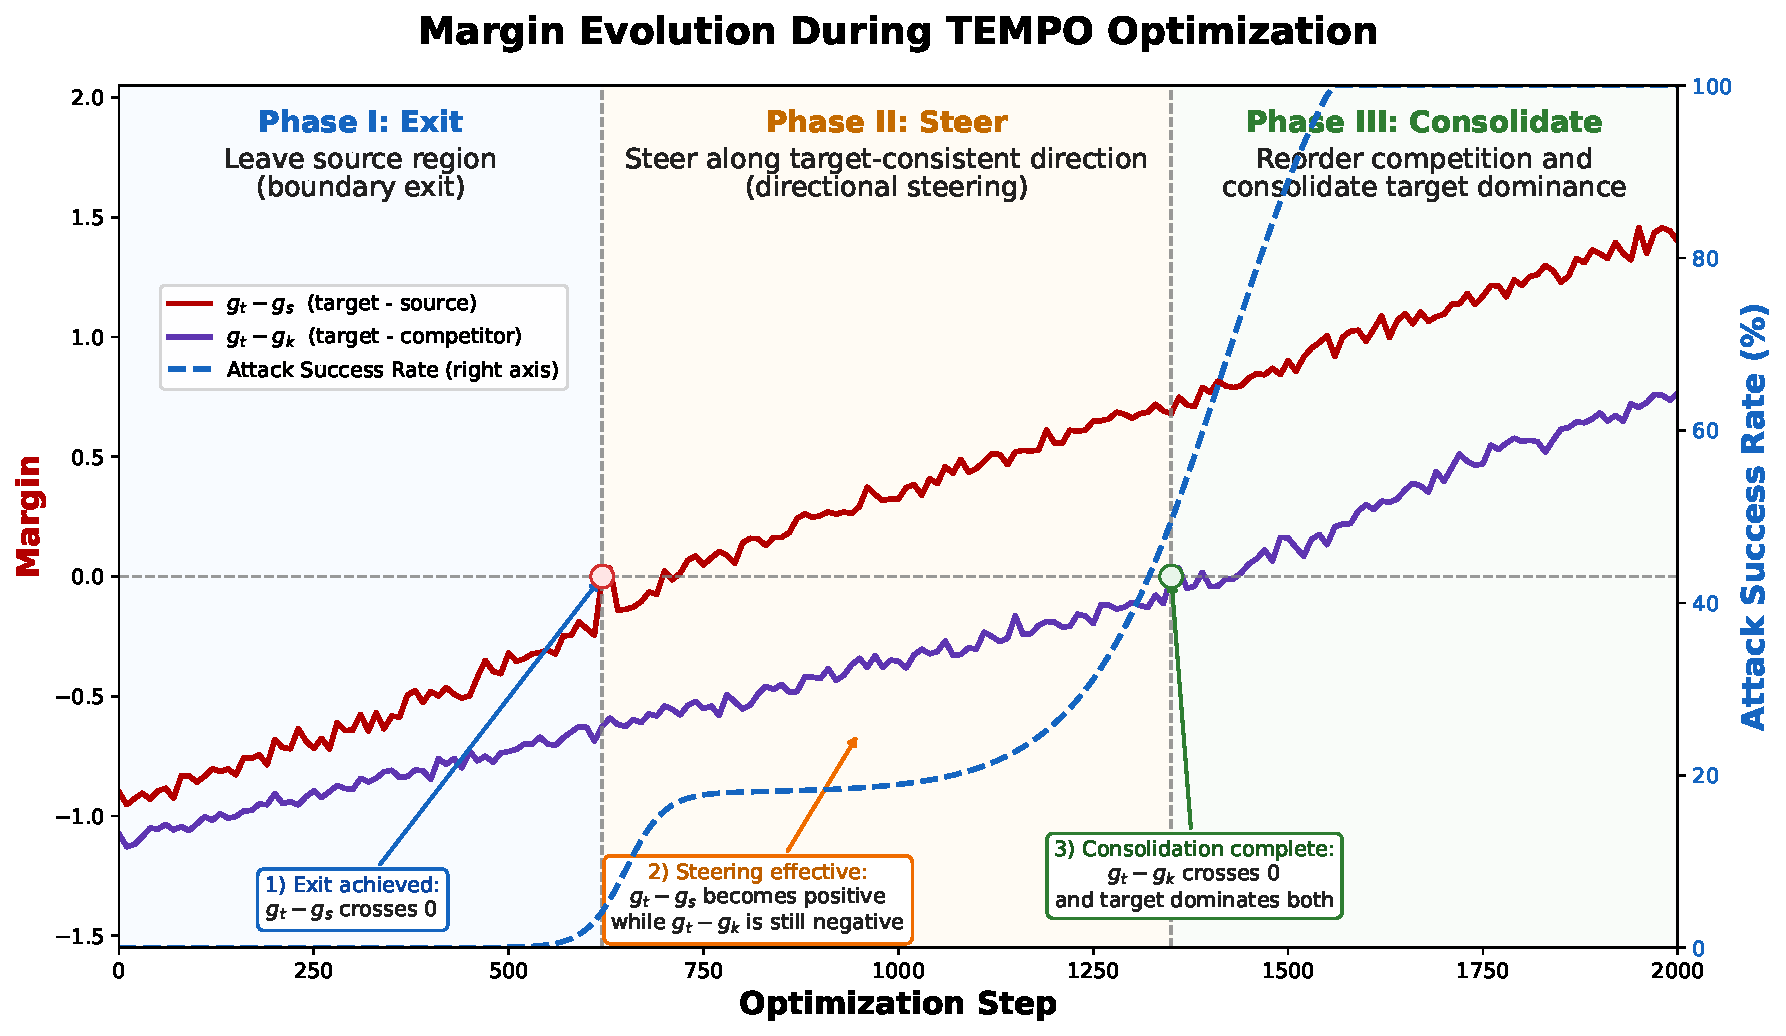
\includegraphics[width=\linewidth]{figure/fig9_margin_evolution.pdf}
    \caption{\textbf{Margin evolution during \textsc{TEMPO} optimization.} The attack first flips the target-source margin, then flips the target-competitor margin, after which the targeted success rate increases rapidly. This shows that stable emotion flipping requires competition-aware margin reordering rather than target-only score maximization.}
    \label{fig:tempo-margin-dynamics}
\end{figure}

This component ties the entire attack together. Topology modeling identifies the relevant competition structure, route planning selects a feasible trajectory, layer-adaptive objectives realize the trajectory, and margin-aware optimization controls the order and effort with which these objectives are applied.

\subsection{Design Rationale}
\label{subsec:tempo-discussion}

TEMPO is not an ad hoc combination of auxiliary losses. Each component operationalizes one structural property revealed in Section~\ref{sec:Observation} and formalized as a challenge in Section~\ref{sec:threat_model}. The topology bank addresses the implicit competition interface by identifying bias centers, competitors, prototypes, and controllable layers. The hardness matrix and route policy address pair-wise transition difficulty by deciding whether a direct or waypoint-assisted route is more feasible. The layer-adaptive objectives address the internal control bottleneck by steering representations before the final decoding step. The margin-aware schedule coordinates these terms under imperceptibility and preservation constraints.

This design also explains why target-only attacks are fragile. A target-only objective ignores the strongest competitor, treats all source--target pairs as equally feasible, and assumes that output-level target increase is enough to change the internal emotion state. TEMPO instead treats emotion flipping as a mechanism-aligned control problem: profile the topology, plan the transition, steer the representation, and consolidate the target. This is the core distinction between classifier-style perturbation and topology-guided emotion manipulation in generative audio-language systems.
